\documentclass{article}
\usepackage{tikz,pgfplots}
% and optionally (as of Pgfplots 1.3):
\pgfplotsset{compat=newest}
\pgfplotsset{plot coordinates/math parser=false}
%\newlength\figureheight
%\newlength\figurewidth

\begin{document}
% Setting the figure dimensions is optional (see above).
%\setlength\figureheight{2cm}
%\setlength\figurewidth{3cm}
\section{Matlab figures}

This is my first figure, \\
% This file was created by matlab2tikz v0.3.2.
% Copyright (c) 2008--2013, Nico Schlömer <nico.schloemer@gmail.com>
% All rights reserved.
% 
% The latest updates can be retrieved from
%   http://www.mathworks.com/matlabcentral/fileexchange/22022-matlab2tikz
% where you can also make suggestions and rate matlab2tikz.
% 
% 
% 
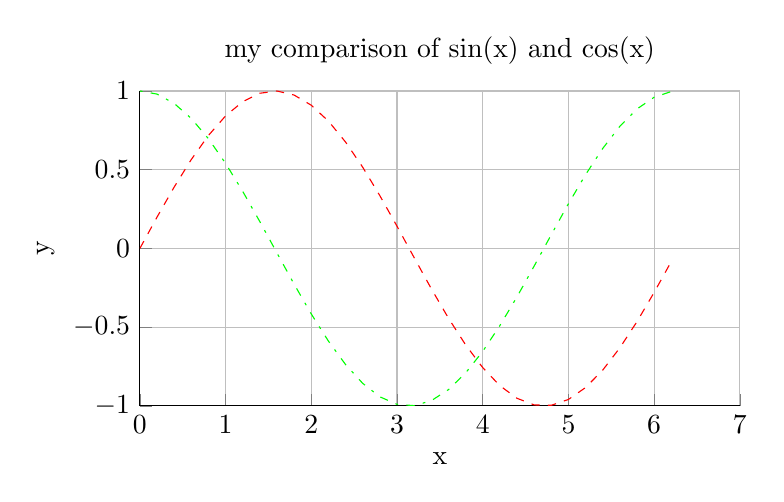
\begin{tikzpicture}

\begin{axis}[%
width=3in,
height=4cm,
scale only axis,
xmin=0, xmax=7,
xlabel={x},
xmajorgrids,
ymin=-1, ymax=1,
ylabel={y},
ymajorgrids,
title={my comparison of sin(x) and cos(x)},
axis x line*=bottom,
axis y line*=left
]
\addplot [
color=red,
dashed,
forget plot
]
table{
0 0
0.2 0.198669330795061
0.4 0.389418342308651
0.6 0.564642473395035
0.8 0.717356090899523
1 0.841470984807897
1.2 0.932039085967226
1.4 0.98544972998846
1.6 0.999573603041505
1.8 0.973847630878195
2 0.909297426825682
2.2 0.80849640381959
2.4 0.675463180551151
2.6 0.515501371821464
2.8 0.334988150155905
3 0.141120008059867
3.2 -0.0583741434275801
3.4 -0.255541102026831
3.6 -0.442520443294852
3.8 -0.611857890942719
4 -0.756802495307928
4.2 -0.871575772413588
4.4 -0.951602073889516
4.6 -0.993691003633464
4.8 -0.996164608835841
5 -0.958924274663138
5.2 -0.883454655720153
5.4 -0.772764487555987
5.6 -0.631266637872322
5.8 -0.464602179413757
6 -0.279415498198926
6.2 -0.0830894028174964
};
\addplot [
color=green,
dash pattern=on 1pt off 3pt on 3pt off 3pt,
forget plot
]
table{
0 1
0.2 0.980066577841242
0.4 0.921060994002885
0.6 0.825335614909678
0.8 0.696706709347165
1 0.54030230586814
1.2 0.362357754476673
1.4 0.169967142900241
1.6 -0.0291995223012888
1.8 -0.227202094693087
2 -0.416146836547142
2.2 -0.588501117255346
2.4 -0.737393715541246
2.6 -0.856888753368947
2.8 -0.942222340668658
3 -0.989992496600445
3.2 -0.998294775794753
3.4 -0.966798192579461
3.6 -0.896758416334147
3.8 -0.790967711914417
4 -0.653643620863612
4.2 -0.490260821340699
4.4 -0.307332869978419
4.6 -0.112152526935055
4.8 0.0874989834394464
5 0.283662185463226
5.2 0.468516671300377
5.4 0.634692875942635
5.6 0.77556587851025
5.8 0.885519516941319
6 0.960170286650366
6.2 0.996542097023218
};
\end{axis}
\end{tikzpicture}% 

This is my second figure, \\
%% This file was created by matlab2tikz v0.3.2.
% Copyright (c) 2008--2013, Nico Schlömer <nico.schloemer@gmail.com>
% All rights reserved.
% 
% The latest updates can be retrieved from
%   http://www.mathworks.com/matlabcentral/fileexchange/22022-matlab2tikz
% where you can also make suggestions and rate matlab2tikz.
% 
% 
% 
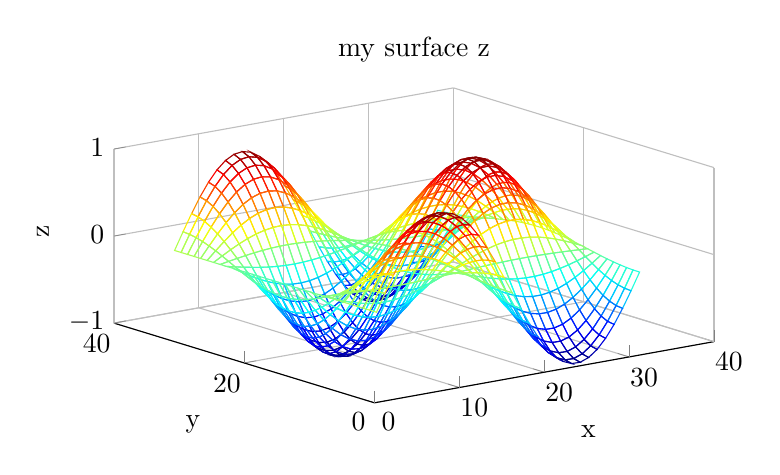
\begin{tikzpicture}

\begin{axis}[%
width=3in,
height=4cm,
view={-37.5}{30},
scale only axis,
xmin=0, xmax=40,
xlabel={x},
xmajorgrids,
ymin=0, ymax=40,
ylabel={y},
ymajorgrids,
zmin=-1, zmax=1,
zlabel={z},
zmajorgrids,
title={my surface z},
axis x line*=bottom,
axis y line*=left,
axis z line*=left
]

\addplot3[%
mesh,
colormap/jet,
shader=flat,
mesh/rows=32]
table[header=false] {
1 1 0
1 2 0
1 3 0
1 4 0
1 5 0
1 6 0
1 7 0
1 8 0
1 9 0
1 10 0
1 11 0
1 12 0
1 13 0
1 14 0
1 15 0
1 16 0
1 17 0
1 18 0
1 19 0
1 20 0
1 21 0
1 22 0
1 23 0
1 24 0
1 25 0
1 26 0
1 27 0
1 28 0
1 29 0
1 30 0
1 31 0
1 32 0
2 1 0.198669330795061
2 2 0.194709171154325
2 3 0.182986571299987
2 4 0.163968874295436
2 5 0.138414255706431
2 6 0.107341497533852
2 7 0.0719893725902818
2 8 0.0337672585371394
2 9 -0.00580104955513251
2 10 -0.0451380881079117
2 11 -0.0826756135293025
2 12 -0.116917123137265
2 13 -0.146497515999063
2 14 -0.170237515197623
2 15 -0.187190681880799
2 16 -0.196681146791742
2 17 -0.198330555043349
2 18 -0.192073149933636
2 19 -0.178158394457944
2 20 -0.157141026006538
2 21 -0.129858940735435
2 22 -0.0973997892907938
2 23 -0.0610576156099381
2 24 -0.0222812674731624
2 25 0.017383364485163
2 26 0.0563549765578437
2 27 0.0930798935535756
2 28 0.126094008923916
2 29 0.154081154071115
2 30 0.175925569836698
2 31 0.19075638829813
2 32 0.19798235152471
3 1 0.389418342308651
3 2 0.381655902095048
3 3 0.358678045449761
3 4 0.321400827006418
3 5 0.271310371829288
3 6 0.210403628296712
3 7 0.141108756070991
3 8 0.0661883230351493
3 9 -0.0113708295707724
3 10 -0.088476663084435
3 11 -0.162055211245177
3 12 -0.229173129528366
3 13 -0.287154638334889
3 14 -0.333688197879862
3 15 -0.366918661989366
3 16 -0.385521236924148
3 17 -0.388754296725379
3 18 -0.376488949501293
3 19 -0.349214175940174
3 20 -0.308017335193378
3 21 -0.254540815297332
3 22 -0.190916556345373
3 23 -0.119681056763956
3 24 -0.0436742511247753
3 25 0.0340737090846813
3 26 0.110463258038739
3 27 0.18244898548176
3 28 0.247161047624691
3 29 0.302019578760614
3 30 0.344837542369245
3 31 0.373907921361407
3 32 0.388071771463568
4 1 0.564642473395035
4 2 0.553387216604087
4 3 0.520070157801479
4 4 0.466019542983613
4 5 0.3933901995967
4 6 0.305077630366427
4 7 0.20460257874158
4 8 0.0959706679630794
4 9 -0.0164872904941532
4 10 -0.128287952708038
4 11 -0.234974179083498
4 12 -0.3322927264428
4 13 -0.416363811409164
4 14 -0.483835785126631
4 15 -0.532018752923211
4 16 -0.558991811923002
4 17 -0.563679631382092
4 18 -0.545895322731917
4 19 -0.506347890236728
4 20 -0.446613965230968
4 21 -0.369074950803317
4 22 -0.276822082770494
4 23 -0.17353319186021
4 24 -0.0633260802061127
4 25 0.0494056424288003
4 26 0.160167718008597
4 27 0.264544412109854
4 28 0.358374555318458
4 29 0.437917435922821
4 30 0.500001930285323
4 31 0.542152925534683
4 32 0.562689994505465
5 1 0.717356090899523
5 2 0.703056729101466
5 3 0.660728714137938
5 4 0.592059530391761
5 5 0.499786801520753
5 6 0.387589150041567
5 7 0.259939542258516
5 8 0.121926965212277
5 9 -0.020946455174186
5 10 -0.162984806493216
5 11 -0.298525467905661
5 12 -0.422164860964297
5 13 -0.528973873234543
5 14 -0.614694366452513
5 15 -0.675908935060267
5 16 -0.710177147381155
5 17 -0.71613283792954
5 18 -0.693538572117526
5 19 -0.643295112022711
5 20 -0.567405505846666
5 21 -0.46889523270413
5 22 -0.351691586318154
5 23 -0.22046710621265
5 24 -0.0804532983066344
5 25 0.0627679287178033
5 26 0.203486796499915
5 27 0.336093287845295
5 28 0.455300800407984
5 29 0.556356906843167
5 30 0.635232819088258
5 31 0.688784003429381
5 32 0.714875543137388
6 1 0.841470984807897
6 2 0.824697588433375
6 3 0.775046101691748
6 4 0.694495972675078
6 5 0.586258480836628
6 6 0.454648713412841
6 7 0.304913536512264
6 8 0.14302241912125
6 9 -0.0245705507867856
6 10 -0.191183970371809
6 11 -0.350175488374015
6 12 -0.495206614697403
6 13 -0.620495416007646
6 14 -0.721047023168179
6 15 -0.792852760910457
6 16 -0.833049961066805
6 17 -0.840036088116589
6 18 -0.813532627220333
6 19 -0.754596187727464
6 20 -0.665576379495873
6 21 -0.550022141361503
6 22 -0.412540256146287
6 23 -0.258611692764578
6 24 -0.0943730972887348
6 25 0.0736278557644808
6 26 0.238693498554501
6 27 0.394243184798046
6 28 0.534075639370005
6 29 0.652616183573421
6 30 0.745138979987224
6 31 0.807955436690964
6 32 0.838561259784653
7 1 0.932039085967226
7 2 0.913460357398178
7 3 0.858464846970514
7 4 0.769245052136615
7 5 0.649357884567166
7 6 0.503582867307326
7 7 0.337731590275575
7 8 0.158416020513201
7 9 -0.0272150960763729
7 10 -0.211761232667584
7 11 -0.387865117163551
7 12 -0.548506043417364
7 13 -0.68727976463104
7 14 -0.79865381046559
7 15 -0.878188049174717
7 16 -0.922711701645892
7 17 -0.930449750357599
7 18 -0.901093703726527
7 19 -0.835813894693496
7 20 -0.737212823242302
7 21 -0.609221402938029
7 22 -0.456942247807927
7 23 -0.28644624722237
7 24 -0.104530538693463
7 25 0.0815524725479631
7 26 0.264384244062611
7 27 0.436675850079211
7 28 0.591558567963483
7 29 0.722857712514062
7 30 0.825338801176127
7 31 0.894916236342497
7 32 0.928816185237383
8 1 0.98544972998846
8 2 0.965806344504366
8 3 0.907659307843046
8 4 0.813326758862602
8 5 0.686569438607313
8 6 0.532440761429901
8 7 0.357085351308263
8 8 0.167494075077952
8 9 -0.0287746613675971
8 10 -0.223896242868115
8 11 -0.410091787710933
8 12 -0.579938267097188
8 13 -0.726664437875308
8 14 -0.844420790637577
8 15 -0.928512751201024
8 16 -0.975587838465511
8 17 -0.98376931725583
8 18 -0.952731017830761
8 19 -0.883710339241364
8 20 -0.779458918135652
8 21 -0.644132929688726
8 22 -0.483127394014113
8 23 -0.302861093736812
8 24 -0.110520677385673
8 25 0.0862258496046672
8 26 0.279534824072673
8 27 0.461699627228049
8 28 0.625457923223269
8 29 0.764281185566188
8 30 0.872634968869334
8 31 0.946199549722546
8 32 0.982042140433664
9 1 0.999573603041505
9 2 0.979648680433328
9 3 0.920668256396454
9 4 0.824983694313743
9 5 0.696409635725337
9 6 0.54007192260825
9 7 0.362203246232278
9 8 0.169894669427464
9 9 -0.02918707171379
9 10 -0.227105216410946
9 11 -0.415969392801751
9 12 -0.588250182168877
9 13 -0.737079293103726
9 14 -0.856523378610742
9 15 -0.941820579928371
9 16 -0.989570366810962
9 17 -0.997869105938673
9 18 -0.966385952770667
9 19 -0.896376041272917
9 20 -0.790630445687789
9 21 -0.653364909211736
9 22 -0.490051775617611
9 23 -0.307201824177415
9 24 -0.112104705438682
9 25 0.0874616741390364
9 26 0.283541232770105
9 27 0.46831689721673
9 28 0.634422244830754
9 29 0.77523517957854
9 30 0.885141934112607
9 31 0.959760872960501
9 32 0.996117174504035
10 1 0.973847630878195
10 2 0.954435514933593
10 3 0.896973066904025
10 4 0.803751133259189
10 5 0.67848617831468
10 6 0.526172120527714
10 7 0.352881240727451
10 8 0.165522099440535
10 9 -0.0284358856158851
10 10 -0.221260221647426
10 11 -0.40526361086889
10 12 -0.57311041880829
10 13 -0.718109122904312
10 14 -0.834479082394519
10 15 -0.917580994220681
10 16 -0.964101847401533
10 17 -0.972187002325799
10 18 -0.941514129380829
10 19 -0.873306059217091
10 20 -0.770282032349002
10 21 -0.636549291616674
10 22 -0.477439339375038
10 23 -0.29929538731948
10 24 -0.109219472652706
10 25 0.0852106777267553
10 26 0.276243747283094
10 27 0.45626385037281
10 28 0.618094153572003
10 29 0.755282993377173
10 30 0.862361083669707
10 31 0.935059558894097
10 32 0.970480160256449
11 1 0.909297426825682
11 2 0.891172017348893
11 3 0.837518391796328
11 4 0.750475550904962
11 5 0.633513618061566
11 6 0.491295496433882
11 7 0.329490973735971
11 8 0.154550685684102
11 9 -0.026551050493101
11 10 -0.206594280073829
11 11 -0.378401247653964
11 12 -0.535122551604325
11 13 -0.670510208099083
11 14 -0.77916673851425
11 15 -0.856760349867682
11 16 -0.900197629735517
11 17 -0.90774687084369
11 18 -0.879107108772224
11 19 -0.815420120456913
11 20 -0.719224905145976
11 21 -0.594356462512304
11 22 -0.445792903318543
11 23 -0.279456987850329
11 24 -0.101980004154043
11 25 0.0795626004913516
11 26 0.257933295329461
11 27 0.426021003638367
11 28 0.577124598919229
11 29 0.705220057663169
11 30 0.805200618158662
11 31 0.873080370965655
11 32 0.90615316454668
12 1 0.80849640381959
12 2 0.792380303688416
12 3 0.74467450134983
12 4 0.667280876598705
12 5 0.563284869024164
12 6 0.436832471269823
12 7 0.292964941390532
12 8 0.137417823802335
12 9 -0.0236077087738419
12 10 -0.183692076499639
12 11 -0.336453220809263
12 12 -0.475801036944758
12 13 -0.596180167214263
12 14 -0.692791475572246
12 15 -0.761783374029087
12 16 -0.800405373309838
12 17 -0.807117736181942
12 18 -0.781652861919774
12 19 -0.725025954701109
12 20 -0.639494550620216
12 21 -0.528468516847846
12 22 -0.396374110987594
12 23 -0.248477520153106
12 24 -0.0906749147062716
12 25 0.0707426134486623
12 26 0.229339856846624
12 27 0.37879404387588
12 28 0.513146907729533
12 29 0.627042223700718
12 30 0.715939344959117
12 31 0.776294223811246
12 32 0.805700701698104
13 1 0.675463180551151
13 2 0.661998887820527
13 3 0.622142788490793
13 4 0.557483819469031
13 5 0.470599729806962
13 6 0.364954313980814
13 7 0.244759321336187
13 8 0.114806546932589
13 9 -0.0197232022042028
13 10 -0.153466649509276
13 11 -0.281091865790433
13 12 -0.397510836419202
13 13 -0.49808230441792
13 14 -0.5787968027291
13 15 -0.636436499014402
13 16 -0.668703480475511
13 17 -0.674311364385922
13 18 -0.653036582110827
13 19 -0.605727292083076
13 20 -0.534269566402978
13 21 -0.441512199095506
13 22 -0.331153133682408
13 23 -0.207592037843536
13 24 -0.0757549025504008
13 25 0.0591023416490009
13 26 0.191603361995081
13 27 0.316465760937791
13 28 0.428711668657369
13 29 0.52386619502548
13 30 0.598135829353302
13 31 0.648559675691566
13 32 0.673127494408416
14 1 0.515501371821464
14 2 0.505225665353528
14 3 0.474808205939729
14 4 0.425461641699051
14 5 0.359153264425682
14 6 0.278526579873326
14 7 0.18679591952287
14 8 0.087618295329649
14 9 -0.0150523938028458
14 10 -0.117122991494997
14 11 -0.214524265119215
14 12 -0.303373133263595
14 13 -0.380127471934039
14 14 -0.441727327860077
14 15 -0.485716909175524
14 16 -0.510342490090486
14 17 -0.514622326404396
14 18 -0.498385794549224
14 19 -0.462280193812696
14 20 -0.407744940558367
14 21 -0.336954183237541
14 22 -0.252730125951448
14 23 -0.158430516079703
14 24 -0.0578147814882645
14 25 0.0451058459960182
14 26 0.146228245740168
14 27 0.24152098677657
14 28 0.327185048233739
14 29 0.399805274309953
14 30 0.45648652575793
14 31 0.494969099950472
14 32 0.513718818093307
15 1 0.334988150155905
15 2 0.328310689940665
15 3 0.308544518561785
15 4 0.276477650896379
15 5 0.233388491765414
15 6 0.180994869967738
15 7 0.121385553866788
15 8 0.056936978787436
15 9 -0.00978149396114482
15 10 -0.0761100094127839
15 11 -0.139404258968159
15 12 -0.197140900634051
15 13 -0.247018156705751
15 14 -0.287047578380463
15 15 -0.31563331893616
15 16 -0.331635755104409
15 17 -0.334416920253788
15 18 -0.323865938106266
15 19 -0.300403443024514
15 20 -0.264964810647259
15 21 -0.218962867414309
15 22 -0.164231565634835
15 23 -0.102952869596176
15 24 -0.0375697675332843
15 25 0.0293111226029023
15 26 0.0950234707775073
15 27 0.156947533036115
15 28 0.212614592429154
15 29 0.259805378966188
15 30 0.296638544907123
15 31 0.321645668159671
15 32 0.333829793634294
16 1 0.141120008059867
16 2 0.138307003364162
16 3 0.129980134897316
16 4 0.116471368628149
16 5 0.0983192564384355
16 6 0.0762474657588767
16 7 0.0511359292323035
16 8 0.0239857645759946
16 9 -0.00412063682250215
16 10 -0.0320627614343072
16 11 -0.058726644927621
16 12 -0.0830492824103153
16 13 -0.104061007080476
16 14 -0.120924147781835
16 15 -0.132966424309348
16 16 -0.139707749099463
16 17 -0.140879366806279
16 18 -0.136434568729079
16 19 -0.126550554940829
16 20 -0.111621369880457
16 21 -0.0922421930445537
16 22 -0.0691856110590366
16 23 -0.0433708170884167
16 24 -0.0158269655050094
16 25 0.0123478572482049
16 26 0.04003040989885
16 27 0.0661170764300914
16 28 0.0895678637685649
16 29 0.109447863026324
16 30 0.124964521367929
16 31 0.135499238590945
16 32 0.140632028763913
17 1 -0.0583741434275801
17 2 -0.0572105469834822
17 3 -0.0537661465694739
17 4 -0.0481782595606276
17 5 -0.0406696573783888
17 6 -0.031539684296999
17 7 -0.0211523235319172
17 8 -0.00992168637763466
17 9 0.00170449710283226
17 10 0.0132627276626609
17 11 0.0242922151235366
17 12 0.0343532486259547
17 13 0.0430447265136009
17 14 0.0500201469906392
17 15 0.0550014220548625
17 16 0.0577899639887825
17 17 0.0582746024252468
17 18 0.0564360163591587
17 19 0.0523475044149791
17 20 0.046172062661877
17 21 0.0381558864748153
17 22 0.0286185555018652
17 23 0.0179402930321301
17 24 0.00654680769307243
17 25 -0.0051076782090617
17 26 -0.0165585370992112
17 27 -0.0273492593687006
17 28 -0.0370496529727386
17 29 -0.0452729938296945
17 30 -0.051691443289854
17 31 -0.0560491180278292
17 32 -0.0581722913032547
18 1 -0.255541102026831
18 2 -0.250447293361216
18 3 -0.235368941441426
18 4 -0.210907172576012
18 5 -0.178037200296062
18 6 -0.138069446669182
18 7 -0.0925972999069371
18 8 -0.0434335910050794
18 9 0.00746167810752838
18 10 0.0580594736606759
18 11 0.106342621216236
18 12 0.150386224047453
18 13 0.18843440269707
18 14 0.218970296350298
18 15 0.240776535288769
18 16 0.252983773579572
18 17 0.25510534715422
18 18 0.247056675569304
18 19 0.229158633961864
18 20 0.202124760770251
18 21 0.167032811208296
18 22 0.125281790565982
18 23 0.0785361802833541
18 24 0.0286595803280778
18 25 -0.0223595866543436
18 26 -0.0724873474766122
18 27 -0.119725266502041
18 28 -0.16219011696696
18 29 -0.198188959288917
18 30 -0.226286633225452
18 31 -0.245362973184053
18 32 -0.254657465689442
19 1 -0.442520443294852
19 2 -0.433699496484775
19 3 -0.407588319367754
19 4 -0.36522788217686
19 5 -0.308306961866806
19 6 -0.239094815906
19 7 -0.160350714142345
19 8 -0.0752139354217741
19 9 0.0129213855527643
19 10 0.100541571661104
19 11 0.184153482584592
19 12 0.260423775287352
19 13 0.32631179388415
19 14 0.3791907909952
19 15 0.416952647875008
19 16 0.438091918454207
19 17 0.44176584672363
19 18 0.427827964756925
19 19 0.396833931924577
19 20 0.350019382508283
19 21 0.289250664861418
19 22 0.216950435989785
19 23 0.136001077861929
19 24 0.0496297859359384
19 25 -0.0387200889394728
19 26 -0.125526316057174
19 27 -0.207328205074872
19 28 -0.280864572818219
19 29 -0.343203756362717
19 30 -0.391860489183116
19 31 -0.424894980887066
19 32 -0.440990250536696
20 1 -0.611857890942719
20 2 -0.59966146930139
20 3 -0.56355843722021
20 4 -0.504988108658548
20 5 -0.426285497786798
20 6 -0.330588229339968
20 7 -0.221711451420837
20 8 -0.103995737584501
20 9 0.0178659581318015
20 10 0.13901539447668
20 11 0.254622725732219
20 12 0.36007905242129
20 13 0.451180163585482
20 14 0.52429414540886
20 15 0.576506174160637
20 16 0.605734721019065
20 17 0.610814536056912
20 18 0.591543103078902
20 19 0.548688713303344
20 20 0.483959836015743
20 21 0.399937007289772
20 22 0.299969952157365
20 23 0.188044041642369
20 24 0.0686214085943792
20 25 -0.0535369434668916
20 26 -0.173560946537732
20 27 -0.286665622373352
20 28 -0.388341844470629
20 29 -0.474536102712418
20 30 -0.541812104024331
20 31 -0.587487766535759
20 32 -0.60974214572026
21 1 -0.756802495307928
21 2 -0.741716831678154
21 3 -0.697061258592184
21 4 -0.624616052830148
21 5 -0.52726937613171
21 6 -0.408902133301636
21 7 -0.274233252782124
21 8 -0.128631557867261
21 9 0.0220982713394149
21 10 0.171947112202917
21 11 0.314940964313378
21 12 0.445379114030349
21 13 0.558061403945999
21 14 0.648495546750919
21 15 0.713076218552917
21 16 0.749228791763343
21 17 0.755511977374338
21 18 0.731675284603331
21 19 0.678669007170068
21 20 0.598606338084833
21 21 0.494679123311691
21 22 0.371030612942356
21 23 0.232590282889815
21 24 0.0848773122395391
21 25 -0.0662194490038801
21 26 -0.21467624978307
21 27 -0.35457458593349
21 28 -0.480337152267551
21 29 -0.586950192132242
21 30 -0.670163380065061
21 31 -0.726659268857526
21 32 -0.754185545706566
22 1 -0.871575772413588
22 2 -0.854202284598722
22 3 -0.802774447288092
22 4 -0.719342526065347
22 5 -0.607232688344985
22 6 -0.470914399573867
22 7 -0.31582223974806
22 8 -0.148139243858208
22 9 0.0254495962038536
22 10 0.198023841176113
22 11 0.362703500501047
22 12 0.512923315838088
22 13 0.642694497195787
22 14 0.746843477090057
22 15 0.821218164353625
22 16 0.86285347490819
22 17 0.870089540309762
22 18 0.842637881465505
22 19 0.78159290938482
22 20 0.689388294466016
22 21 0.569699943737417
22 22 0.42729945404414
22 23 0.267863883539526
22 24 0.0977494252915562
22 25 -0.0762619940766393
22 26 -0.247233088399638
22 27 -0.408347779677269
22 28 -0.553182933595104
22 29 -0.675964429620194
22 30 -0.771797356965438
22 31 -0.836861159235869
22 32 -0.868561947955668
23 1 -0.951602073889516
23 2 -0.932633388023526
23 3 -0.876483552071885
23 4 -0.785391082802929
23 5 -0.662987549507503
23 6 -0.51415279479141
23 7 -0.344820390649951
23 8 -0.161741085676945
23 9 0.0277863259784896
23 10 0.216205984501984
23 11 0.396006192700822
23 12 0.560018883666484
23 13 0.701705388982145
23 14 0.815417114798492
23 15 0.896620733445329
23 16 0.942078912900044
23 17 0.949979378999357
23 18 0.920007165091251
23 19 0.853357168761452
23 20 0.752686515037404
23 21 0.622008625198466
23 22 0.466533214334587
23 23 0.292458596445881
23 24 0.106724577223348
23 25 -0.0832642141042016
23 26 -0.269933523970839
23 27 -0.445841436061252
23 28 -0.603975057029913
23 29 -0.738030098428298
23 30 -0.842662208791002
23 31 -0.91370003606358
23 32 -0.948311526245501
24 1 -0.993691003633464
24 2 -0.973883341362678
24 3 -0.915250023538363
24 4 -0.820128575514041
24 5 -0.692311189249353
24 6 -0.536893540583587
24 7 -0.360071640720294
24 8 -0.168894820813253
24 9 0.0290153026211854
24 10 0.225768677503199
24 11 0.413521367667421
24 12 0.58478826584488
24 13 0.73274150126919
24 14 0.851482645337417
24 15 0.936277863344911
24 16 0.983746637536496
24 17 0.991996537681533
24 18 0.960698666295304
24 19 0.891100770743835
24 20 0.785977499493902
24 21 0.649519785634574
24 22 0.487167767600206
24 23 0.305393908018409
24 24 0.111444957050124
24 25 -0.0869469526708514
24 26 -0.281872561765815
24 27 -0.465560801323482
24 28 -0.630688600894447
24 29 -0.770672836200719
24 30 -0.87993277752644
24 31 -0.954112575800633
24 32 -0.990254916553998
25 1 -0.996164608835841
25 2 -0.976307639148301
25 3 -0.917528364804835
25 4 -0.822170129984788
25 5 -0.694034566590125
25 6 -0.538230035178238
25 7 -0.360967970746889
25 8 -0.169315252422164
25 9 0.0290875307114568
25 10 0.226330685786623
25 11 0.414550750647257
25 12 0.586243985270127
25 13 0.734565522200152
25 14 0.853602249815609
25 15 0.938608549428584
25 16 0.9861954881264
25 17 0.994465924832444
25 18 0.963090143334117
25 19 0.893318997027754
25 20 0.787934041341005
25 21 0.651136641895643
25 22 0.488380479318396
25 23 0.306154128204448
25 24 0.11172237812421
25 25 -0.0871633906114898
25 26 -0.282574230023494
25 27 -0.46671972659901
25 28 -0.632258580494289
25 29 -0.772591279992588
25 30 -0.882123203210352
25 31 -0.956487658016859
25 32 -0.992719968269582
26 1 -0.958924274663138
26 2 -0.939809632277997
26 3 -0.883227745594726
26 4 -0.791434355880919
26 5 -0.668088975913673
26 6 -0.518108996753427
26 7 -0.347473646880108
26 8 -0.162985619222179
26 9 0.0280001307432735
26 10 0.217869603855514
26 11 0.399053303389328
26 12 0.564328007002529
26 13 0.707104733816546
26 14 0.821691426291319
26 15 0.903519874597098
26 16 0.949327836724532
26 17 0.957289093778984
26 18 0.927086255564893
26 19 0.859923413931287
26 20 0.758478139429494
26 21 0.626794735024827
26 22 0.470123002499885
26 23 0.294708949424196
26 24 0.107545780542836
26 25 -0.0839048992284331
26 26 -0.272010555444685
26 27 -0.449272009194302
26 28 -0.608622405697152
26 29 -0.743708947503921
26 30 -0.849146160483007
26 31 -0.9207305956793
26 32 -0.955608407559272
27 1 -0.883454655720153
27 2 -0.865844381109563
27 3 -0.813715623354081
27 4 -0.729146591523611
27 5 -0.615508786044221
27 6 -0.477332587615542
27 7 -0.320126645228717
27 8 -0.15015826371467
27 9 0.025796453921878
27 10 0.200722748345979
27 11 0.367646860210787
27 12 0.519914051935747
27 13 0.651453911093696
27 14 0.757022358598035
27 15 0.832410713587266
27 16 0.874613480249681
27 17 0.881948167456981
27 18 0.854122364376154
27 19 0.792245397966634
27 20 0.698784107615108
27 21 0.577464500033737
27 22 0.433123205130627
27 23 0.271514654838271
27 24 0.0990816720715541
27 25 -0.0773013842903595
27 26 -0.250602678399241
27 27 -0.413913234542827
27 28 -0.560722376203934
27 29 -0.685177286187571
27 30 -0.782316339972869
27 31 -0.84826691002542
27 32 -0.880399755236286
28 1 -0.772764487555987
28 2 -0.757360646796237
28 3 -0.711763227038448
28 4 -0.637790053517383
28 5 -0.53839020322548
28 6 -0.417526434519511
28 7 -0.280017204450105
28 8 -0.13134457208466
28 9 0.0225643538880351
28 10 0.17557371027715
28 11 0.321583496892398
28 12 0.454772764301953
28 13 0.569831676717236
28 14 0.662173198389643
28 15 0.728115964250618
28 16 0.765031044319716
28 17 0.771446750846851
28 18 0.747107309858722
28 19 0.692983058059976
28 20 0.611231758570876
28 21 0.505112577720909
28 22 0.378856152372123
28 23 0.237495927777984
28 24 0.0866674900050767
28 25 -0.0676161070992536
28 26 -0.219204063388501
28 27 -0.362053045408873
28 28 -0.490468115033246
28 29 -0.599329768672882
28 30 -0.684298035729984
28 31 -0.741985499529855
28 32 -0.770092342934116
29 1 -0.631266637872322
29 2 -0.618683333484873
29 3 -0.58143507695954
29 4 -0.521006838740318
29 5 -0.439807701992674
29 6 -0.341074820060043
29 7 -0.228744361375454
29 8 -0.107294586847399
29 9 0.0184326842706125
29 10 0.143425102434454
29 11 0.262699614368317
29 12 0.371501121673887
29 13 0.465492051597901
29 14 0.54092528236982
29 15 0.594793529122093
29 16 0.624949234847789
29 17 0.630190186721457
29 18 0.610307444530674
29 19 0.566093670462965
29 20 0.499311528165777
29 21 0.412623410909263
29 22 0.309485300368266
29 23 0.194008987538928
29 24 0.0707981486071771
29 25 -0.0552351890930653
29 26 -0.179066474108886
29 27 -0.295758943878921
29 28 -0.400660437877822
29 29 -0.489588864575659
29 30 -0.558998928229869
29 31 -0.60612346863868
29 32 -0.629083779086079
30 1 -0.464602179413757
30 2 -0.455341068035624
30 3 -0.427926945186742
30 4 -0.38345272543483
30 5 -0.32369145557488
30 6 -0.251025628848616
30 7 -0.168352202457338
30 8 -0.0789671050201814
30 9 0.0135661616990194
30 10 0.105558588361779
30 11 0.193342727215943
30 12 0.273418901664265
30 13 0.342594727326471
30 14 0.398112382330351
30 15 0.43775855296699
30 16 0.459952671523834
30 17 0.463809928531611
30 18 0.449176547325699
30 19 0.416635914636474
30 20 0.367485322801351
30 21 0.303684250813134
30 22 0.227776246076068
30 23 0.142787521197459
30 24 0.0521063084407866
30 25 -0.0406522184024551
30 26 -0.131790069583484
30 27 -0.217673866577834
30 28 -0.294879693421334
30 29 -0.360329597434807
30 30 -0.411414297484354
30 31 -0.446097207786092
30 32 -0.462995630154543
31 1 -0.279415498198926
31 2 -0.273845791115627
31 3 -0.257358716510914
31 4 -0.230611562021305
31 5 -0.194670652290772
31 6 -0.150968837972175
31 7 -0.101248372493344
31 8 -0.0474914539109188
31 9 0.00815879907098526
31 10 0.0634837864805085
31 11 0.116277875657727
31 12 0.164436332868527
31 13 0.206039232396714
31 14 0.239427997923641
31 15 0.263271524732091
31 16 0.276619246650812
31 17 0.278939032128076
31 18 0.270138398637411
31 19 0.250568199664085
31 20 0.221008637283831
31 21 0.182638157968156
31 22 0.136986471642326
31 23 0.0858735669779258
31 24 0.0313371541878268
31 25 -0.0244485720496325
31 26 -0.0792596108714035
31 27 -0.130910819125897
31 28 -0.17734302613482
31 29 -0.216705126330029
31 30 -0.247427876991031
31 31 -0.268286459000217
31 32 -0.278449306515945
32 1 -0.0830894028174964
32 2 -0.0814331466742161
32 3 -0.0765304079501894
32 4 -0.0685766433668563
32 5 -0.057888944418599
32 6 -0.0448933959355
32 7 -0.0301080894257558
32 8 -0.0141224684021771
32 9 0.00242617087057026
32 10 0.0188780863669329
32 11 0.0345773921330923
32 12 0.0488982063901761
32 13 0.0612696034656969
32 14 0.0711983747984548
32 15 0.0782886916074625
32 16 0.0822578853363333
32 17 0.0829477167566125
32 18 0.0803306844664623
32 19 0.0745111212847681
32 20 0.0657210348308904
32 21 0.0543108581130235
32 22 0.040735478870014
32 23 0.0255361046326941
32 24 0.00931868648750689
32 25 -0.00727023828112161
32 26 -0.0235693215920454
32 27 -0.0389287704283896
32 28 -0.0527362520345928
32 29 -0.0644413056910436
32 30 -0.0735772878458921
32 31 -0.0797799757208832
32 32 -0.0828020877241547
};
\end{axis}
\end{tikzpicture}%

This is my third figure, \\
% This file was created by matlab2tikz v0.3.2.
% Copyright (c) 2008--2013, Nico Schlömer <nico.schloemer@gmail.com>
% All rights reserved.
% 
% The latest updates can be retrieved from
%   http://www.mathworks.com/matlabcentral/fileexchange/22022-matlab2tikz
% where you can also make suggestions and rate matlab2tikz.
% 
% 
% 

% defining custom colors
\definecolor{mycolor1}{rgb}{0,0,0.5625}
\definecolor{mycolor2}{rgb}{0,0.5625,1}
\definecolor{mycolor3}{rgb}{0.0625,1,0.9375}
\definecolor{mycolor4}{rgb}{0.5625,1,0.4375}
\definecolor{mycolor5}{rgb}{1,0.9375,0}
\definecolor{mycolor6}{rgb}{1,0.4375,0}
\definecolor{mycolor7}{rgb}{0.9375,0,0}

\begin{tikzpicture}

\begin{axis}[%
width=3in,
height=4cm,
unbounded coords=jump,
scale only axis,
xmin=1, xmax=32,
xlabel={x},
ymin=1, ymax=32,
ylabel={y},
title={my surface z}
]

\addplot [draw=mycolor1,forget plot] table{
21.4005586239166 32 
21.6655124598197 31 
22 30.4334613417971 
22.3979778734878 30 
23 29.5922646628925 
24 29.2684164337216 
25 29.2502349927055 
26 29.533882212035 
26.735392675124 30 
27 30.2681350595308 
27.4541425428997 31 
27.7288699241357 32 
NaN NaN 
};

\addplot [draw=mycolor1,forget plot] table{
21.3763724952482 1 
21.5181396065765 2 
21.9737549560058 3 
22 3.0332540261261 
23 3.83962541234954 
23.4205518607392 4 
24 4.15747916697622 
25 4.17302089597486 
25.7213135387404 4 
26 3.90668561052395 
27 3.16218257507755 
27.1345296810054 3 
27.6069516460356 2 
27.7539482241673 1 
NaN NaN 
};

\addplot [draw=mycolor1,forget plot] table{
6 18.2296139253877 
5.88722251940949 18 
5.67687620739449 17 
5.73102299788334 16 
6 15.1778044008474 
6.08375478931307 15 
7 14.0169259121136 
7.02941399081503 14 
8 13.622773722219 
9 13.5267795942276 
10 13.703711485803 
10.6233524015752 14 
11 14.2684919688923 
11.5976222065034 15 
12 15.9895040827149 
12.0030779611524 16 
12.0535948395072 17 
12 17.2795119311669 
11.8117358794224 18 
11.170587563124 19 
11 19.16030028528 
10 19.7115433306733 
9 19.9113953232722 
8 19.8029659294187 
7 19.3632201371283 
6.55903834235957 19 
6 18.2296139253877 
NaN NaN 
};

\addplot [draw=blue,forget plot] table{
19.9422694144581 32 
20 31.562236913486 
20.0899051404598 31 
20.4533487922411 30 
21 29.156823794304 
21.1466036022555 29 
22 28.3813039254329 
22.9217387114163 28 
23 27.9748626699018 
24 27.8141524263378 
25 27.8051298548032 
26 27.9458902777377 
26.1800083588335 28 
27 28.3155972215257 
27.9921927698491 29 
28 29.007888019261 
28.6727744308147 30 
29 30.8700577536554 
29.0382653984793 31 
29.1751105017015 32 
NaN NaN 
};

\addplot [draw=blue,forget plot] table{
19.9299747863959 1 
20 1.97224344085787 
20.002383089895 2 
20.2729647389118 3 
20.7942282382214 4 
21 4.25286998657801 
21.9095499155201 5 
22 5.05305735870209 
23 5.42320457763816 
24 5.59395564172942 
25 5.6035419235756 
26 5.45398710077778 
27 5.11223920053225 
27.2011030996339 5 
28 4.3801821975225 
28.3235914817855 4 
28.8575524702129 3 
29 2.50158947633337 
29.1143815009146 2 
29.1876023128236 1 
NaN NaN 
};

\addplot [draw=blue,forget plot] table{
5 19.5705012083246 
4.6838554922248 19 
4.36645547624582 18 
4.23823945353753 17 
4.2712444824938 16 
4.4724522970722 15 
4.88770804097349 14 
5 13.8285781392421 
5.77605910710599 13 
6 12.8364146213124 
7 12.3710641765046 
8 12.1367290701885 
9 12.078948384206 
10 12.1854470449191 
11 12.4791976615548 
11.9486098387642 13 
12 13.0395381539766 
12.8139983497292 14 
13 14.3678575467496 
13.2417502532574 15 
13.4338409371429 16 
13.4653504418664 17 
13.3429441449802 18 
13.0399261619937 19 
13 19.0801493754323 
12.3753343458686 20 
12 20.3557233315313 
11 20.9548041333049 
10.8662441555238 21 
10 21.2297109080969 
9 21.3267643455079 
8 21.274108151026 
7 21.0605559108215 
6.84423111551639 21 
6 20.5674943693508 
5.33201796970661 20 
5 19.5705012083246 
NaN NaN 
};

\addplot [draw=mycolor2,forget plot] table{
18.7800158969862 32 
18.8613340250266 31 
19 30.2463943108261 
19.0542809147171 30 
19.4324619578946 29 
20 28.1352544330351 
20.1267255451235 28 
21 27.3611998020607 
21.8447594592011 27 
22 26.9481873464731 
23 26.7394009427064 
24 26.6430865607871 
25 26.6376792925172 
26 26.722037655948 
27 26.9148050507489 
27.2682835287563 27 
28 27.2955023479886 
29 27.993704209038 
29.0062434602934 28 
29.6930943255158 29 
30 29.7765613290617 
30.0696051383402 30 
30.2592487130326 31 
30.3413540238163 32 
NaN NaN 
};

\addplot [draw=mycolor2,forget plot] table{
18.7725928276007 1 
18.8161031850621 2 
18.9559380630732 3 
19 3.17913694642853 
19.2487983791848 4 
19.7772010172713 5 
20 5.27467343857785 
20.8863275503927 6 
21 6.06610386354512 
22 6.45724038954332 
23 6.67413437711572 
24 6.77418883458115 
25 6.77980607763808 
26 6.69217191420835 
27 6.49191898500411 
28 6.12745642245735 
28.2292487168967 6 
29 5.40318586081419 
29.3428262902113 5 
29.8797035278151 4 
30 3.62793558476181 
30.1637288808329 3 
30.3049174004678 2 
30.3488489506371 1 
NaN NaN 
};

\addplot [draw=mycolor2,forget plot] table{
4 20.6011678840007 
3.6636717269509 20 
3.32320132116256 19 
3.1387849232018 18 
3.06428859088188 17 
3.08346523942719 16 
3.2003714099945 15 
3.44164414051592 14 
3.8733541046675 13 
4 12.80535743751 
4.75337337782942 12 
5 11.8207297818602 
6 11.3435435750177 
7 11.0755404187428 
7.54596044020988 11 
8 10.9458000581085 
9 10.9154450933633 
10 10.9713939461052 
10.1959474237905 11 
11 11.1378163134278 
12 11.456029961237 
12.9682059368339 12 
13 12.0247501963562 
13.8315242568067 13 
14 13.3226067296297 
14.2697659389833 14 
14.5039693074146 15 
14.6174500927404 16 
14.6360648598333 17 
14.5637512919992 18 
14.384738348833 19 
14.0542438262466 20 
14 20.1094060983592 
13.3970255054562 21 
13 21.376155768809 
12 21.9725507754186 
11.9266293480398 22 
11 22.275303762207 
10 22.4347009173283 
9 22.4924900165864 
8 22.4611366288998 
7 22.3339799620658 
6 22.0814680256269 
5.79391075956621 22 
5 21.5878249937484 
4.30980727170669 21 
4 20.6011678840007 
NaN NaN 
};

\addplot [draw=mycolor3,forget plot] table{
17.7218239703825 32 
17.7603821804452 31 
17.8494423973813 30 
18 29.0644551828445 
18.0124886614858 29 
18.3186016970697 28 
18.9163474970788 27 
19 26.9104152096868 
20 26.233757386836 
20.6430465392534 26 
21 25.9011412767483 
22 25.72373640944 
23 25.6253614264669 
24 25.5799804748799 
25 25.5774327039792 
26 25.6171802757388 
27 25.7080074983892 
28 25.8733140556902 
28.4784558249056 26 
29 26.1793905462141 
30 26.794211863048 
30.2037026948324 27 
30.8072348451913 28 
31 28.5756037851847 
31.1097117244262 29 
31.2728082615322 30 
31.3622499227203 31 
31.4009732773121 32 
NaN NaN 
};

\addplot [draw=mycolor3,forget plot] table{
17.7183042106983 1 
17.73893529928 2 
17.8052401040063 3 
17.9329733581212 4 
18 4.3318278604897 
18.1685947639661 5 
18.6130198166922 6 
19 6.49647929216769 
19.6461670380149 7 
20 7.18443970404005 
21 7.50983783413737 
22 7.69072143620419 
23 7.79102545572425 
24 7.83729628308562 
25 7.83989401326494 
26 7.79936703076228 
27 7.70675877571258 
28 7.53821071959914 
29 7.23667694309975 
29.4759618117714 7 
30 6.61719504169479 
30.5099666739425 6 
30.9586938883221 5 
31 4.85171917602575 
31.1889195383039 4 
31.3171998730036 3 
31.3837886607193 2 
31.4045081121011 1 
NaN NaN 
};

\addplot [draw=mycolor3,forget plot] table{
3 21.8572330145097 
2.56256019177627 21 
2.28406695673067 20 
2.12768703491221 19 
2.04298357345166 18 
2.00876700006997 17 
2.01757493975951 16 
2.07127058408749 15 
2.18208847044241 14 
2.38037522105135 13 
2.74011965625495 12 
3 11.5653451377131 
3.52036925205738 11 
4 10.672177184706 
5 10.2730929089548 
6 10.0554496852346 
6.42843549843854 10 
7 9.93626941812585 
8 9.87753152324643 
9 9.86304835035504 
10 9.88974305793047 
11 9.96337390698231 
11.2879321220103 10 
12 10.1067543947387 
13 10.3646093761613 
14 10.8508821848136 
14.1933474964047 11 
14.9730863289307 12 
15 12.0573227076052 
15.3288968535606 13 
15.5239933829129 14 
15.6330283282715 15 
15.6858600672432 16 
15.6945262966251 17 
15.6608602312295 18 
15.5775195576629 19 
15.4236556211495 20 
15.149643043715 21 
15 21.3464720698717 
14.5958303249544 22 
14 22.5591765016119 
13.1544304889504 23 
13 23.0575864897751 
12 23.3072035472154 
11 23.447703055323 
10 23.5223985768715 
9 23.5494792791942 
8 23.5347866854412 
7 23.4751994641993 
6 23.3568691792253 
5 23.1461791984573 
4.56391648778841 23 
4 22.7437593926458 
3.10573759375708 22 
3 21.8572330145097 
NaN NaN 
};

\addplot [draw=mycolor4,forget plot] table{
16.7073891991703 32 
16.7073891991703 31 
16.7073891991703 30 
16.7073891991703 29 
16.7073891991703 28 
16.7073891991703 27 
16.7073891991703 26 
16.7073891991703 25 
16 24.5617414399955 
15 24.5617414399955 
14 24.5617414399955 
13 24.5617414399955 
12 24.5617414399955 
11 24.5617414399955 
10 24.5617414399955 
9 24.5617414399955 
8 24.5617414399955 
7 24.5617414399955 
6 24.5617414399955 
5 24.5617414399955 
4 24.5617414399955 
3 24.5617414399955 
2 24.5617414399955 
1 24 
1 23 
1 22 
1 21 
1 20 
1 19 
1 18 
1 17 
1 16 
1 15 
1 14 
1 13 
1 12 
1 11 
1 10 
1 9 
2 8.85339151874766 
3 8.85339151874766 
4 8.85339151874766 
5 8.85339151874766 
6 8.85339151874766 
7 8.85339151874766 
8 8.85339151874766 
9 8.85339151874766 
10 8.85339151874766 
11 8.85339151874766 
12 8.85339151874766 
13 8.85339151874766 
14 8.85339151874766 
15 8.85339151874766 
16 8.85339151874766 
16.7073891991703 9 
16.7073891991703 10 
16.7073891991703 11 
16.7073891991703 12 
16.7073891991703 13 
16.7073891991703 14 
16.7073891991703 15 
16.7073891991703 16 
16.7073891991703 17 
16.7073891991703 18 
16.7073891991703 19 
16.7073891991703 20 
16.7073891991703 21 
16.7073891991703 22 
16.7073891991703 23 
16.7073891991703 24 
17 24.5617414399955 
18 24.5617414399955 
19 24.5617414399955 
20 24.5617414399955 
21 24.5617414399955 
22 24.5617414399955 
23 24.5617414399955 
24 24.5617414399955 
25 24.5617414399955 
26 24.5617414399955 
27 24.5617414399955 
28 24.5617414399955 
29 24.5617414399955 
30 24.5617414399955 
31 24.5617414399955 
32 24.5617414399955 
NaN NaN 
};

\addplot [draw=mycolor4,forget plot] table{
16.7073891991703 1 
16.7073891991703 2 
16.7073891991703 3 
16.7073891991703 4 
16.7073891991703 5 
16.7073891991703 6 
16.7073891991703 7 
16.7073891991703 8 
17 8.85339151874766 
18 8.85339151874766 
19 8.85339151874766 
20 8.85339151874766 
21 8.85339151874766 
22 8.85339151874766 
23 8.85339151874766 
24 8.85339151874766 
25 8.85339151874766 
26 8.85339151874766 
27 8.85339151874766 
28 8.85339151874766 
29 8.85339151874766 
30 8.85339151874766 
31 8.85339151874766 
32 8.85339151874766 
NaN NaN 
};

\addplot [draw=mycolor5,forget plot] table{
2.01061420712389 32 
2.05046974790364 31 
2.14252648762753 30 
2.31039161073441 29 
2.61045509883782 28 
3 27.271217048832 
3.21378796894192 27 
4 26.3816204597624 
4.91950898723263 26 
5 25.9752215423925 
6 25.7655872057899 
7 25.6478498046088 
8 25.5885611400528 
9 25.5739421622868 
10 25.6008871790619 
11 25.6752084450753 
12 25.8150039923897 
12.7774929007596 26 
13 26.0672471302491 
14 26.5642796468546 
14.4909458575973 27 
15 27.7733921538753 
15.1025187143654 28 
15.397754502609 29 
15.5629188558341 30 
15.6534945012994 31 
15.6927088091525 32 
NaN NaN 
};

\addplot [draw=mycolor5,forget plot] table{
2.00697602149746 1 
2.02830126431765 2 
2.0968369625353 3 
2.22886793363169 4 
2.46341267217046 5 
2.89905479132146 6 
3 6.15013561555931 
3.92751139326642 7 
4 7.04236857023499 
5 7.43430492743016 
6 7.64804998694813 
7 7.76809610263122 
8 7.82854735951795 
9 7.84345300104274 
10 7.81597961902128 
11 7.74020098616493 
12 7.59766418582344 
13 7.34442759334384 
13.7721996973253 7 
14 6.85605597488687 
14.8051389640286 6 
15 5.63726252585377 
15.2471953860151 5 
15.4779665511394 4 
15.6078732854461 3 
15.6753063177487 2 
15.6962884602723 1 
NaN NaN 
};

\addplot [draw=mycolor5,forget plot] table{
31 20.5475208456739 
31.1352885674837 20 
31.2872261662501 19 
31.3695234355662 18 
31.4027680102991 17 
31.3942102799272 16 
31.342039981026 15 
31.2343701257317 14 
31.0417161558077 13 
31 12.8548362622508 
30.6736756389168 12 
30 11.0831367486012 
29.9040142506766 11 
29 10.4743251231824 
28 10.1672921404044 
27.0287386079738 10 
27 9.99586826927102 
26 9.90588479778974 
25 9.86650646621127 
24 9.86903056926647 
23 9.91398994866577 
22.1086867916763 10 
22 10.0120000176827 
21 10.196182474862 
20 10.5275150361227 
19.2248714007359 11 
19 11.2077678851603 
18.4508804075836 12 
18.0838832037896 13 
18 13.3787541780919 
17.8877166050329 14 
17.7805059322589 15 
17.7285581254311 16 
17.7200368914414 17 
17.7531396871447 18 
17.8350859810885 19 
17.9863756075014 20 
18 20.0605483820869 
18.2697411859749 21 
18.8150901443845 22 
19 22.2093955576894 
20 22.8931797087679 
20.2683943251512 23 
21 23.2206325060443 
22 23.3989307213418 
23 23.4978010858372 
24 23.5434105598006 
25 23.5459711603719 
26 23.5060234339387 
27 23.4147388376099 
28 23.2485998551178 
28.8622342149588 23 
29 22.948119122318 
30 22.3268227181399 
30.305940247669 22 
30.8565683400118 21 
31 20.5475208456739 
NaN NaN 
};

\addplot [draw=mycolor6,forget plot] table{
3.06831033055221 32 
3.15508382413376 31 
3.3555097814106 30 
3.72098577038222 29 
4 28.5233082378369 
4.42945483592287 28 
5 27.5360963481316 
6 27.0411693781646 
6.13566942269143 27 
7 26.7871292111835 
8 26.6612977580778 
9 26.630271132179 
10 26.6874579593771 
11 26.8451938937109 
11.5509777417228 27 
12 27.1578377677696 
13 27.7442074349018 
13.2827994129773 28 
13.9984304026689 29 
14 29.0034354514954 
14.3533765359892 30 
14.5479299536666 31 
14.6321609583203 32 
NaN NaN 
};

\addplot [draw=mycolor6,forget plot] table{
3.06038927187565 1 
3.1068185959992 2 
3.25603453569148 3 
3.54349239973875 4 
4 4.90899270053856 
4.06212416828893 5 
5 5.88938404864263 
5.18507203647779 6 
6 6.36496910441511 
7 6.62455272676312 
8 6.75527046093435 
9 6.78750191130995 
10 6.72809440792927 
11 6.56423327921637 
12 6.25601656816327 
12.5124292644527 6 
13 5.66827064151219 
13.6334855893852 5 
14 4.38398830956276 
14.1709018637632 4 
14.4499371277005 3 
14.5947809963965 2 
14.6398499276438 1 
NaN NaN 
};

\addplot [draw=mycolor6,forget plot] table{
30 19.3384682465733 
30.1001754894938 19 
30.2746707765132 18 
30.3451594046059 17 
30.3270144086675 16 
30.216397478649 15 
30 14.0476116013057 
29.986782582882 14 
29.5329005491874 13 
29 12.3032088133307 
28.6577601038399 12 
28 11.5887599251257 
27 11.2124761048175 
26 11.0057280188073 
25.9389127386649 11 
25 10.922692882621 
24 10.9279830949128 
23.2280198346173 11 
23 11.0243505991863 
22 11.248279492391 
21 11.6521024399011 
20.468006081422 12 
20 12.4382048371151 
19.5901270777548 13 
19.1434095654707 14 
19 14.5510642411212 
18.9037744242046 15 
18.7942180314107 16 
18.7762470001957 17 
18.8460598202182 18 
19 18.8978491088091 
19.0208493143691 19 
19.3731555044267 20 
20 20.999250290532 
20.0006648860388 21 
21 21.7657117989443 
21.5148388786832 22 
22 22.1712256177071 
23 22.382210888305 
24 22.4795396202774 
25 22.4850038360431 
26 22.3997570392472 
27 22.2049594843262 
27.6103741302855 22 
28 21.8325325022511 
29 21.1223932728945 
29.1158757869817 21 
29.7533519446398 20 
30 19.3384682465733 
NaN NaN 
};

\addplot [draw=mycolor7,forget plot] table{
4.24516129047689 32 
4.39450759890655 31 
4.73946175019525 30 
5 29.5533133236066 
5.45339103553763 29 
6 28.5561334400226 
7 28.0642915996552 
7.24901453056633 28 
8 27.8445396425961 
9 27.7927685933945 
10 27.8881905723817 
10.4416487737139 28 
11 28.1785808904162 
12 28.7625694834759 
12.2620979315441 29 
12.9841755941059 30 
13 30.0369700207753 
13.316163120408 31 
13.4587422472781 32 
NaN NaN 
};

\addplot [draw=mycolor7,forget plot] table{
4.23152831543609 1 
4.31143806522875 2 
4.56825439049244 3 
5 3.88436633180919 
5.07751606197214 4 
6 4.87304288994536 
6.21777573718532 5 
7 5.33858946131481 
8 5.56166989941571 
9 5.61667548925404 
10 5.51529175609289 
11 5.23564942131145 
11.4772065360828 5 
12 4.64695634157378 
12.6127748626199 4 
13 3.34245501940095 
13.1502891453411 3 
13.395468606468 2 
13.4717574848048 1 
NaN NaN 
};

\addplot [draw=mycolor7,forget plot] table{
29 18.2331274528813 
29.063969385819 18 
29.1814529382868 17 
29.1512106333924 16 
29 15.1726529276173 
28.9609482764631 15 
28.5127774598574 14 
28 13.3267037702691 
27.6303908669834 13 
27 12.6088340718693 
26 12.2498445915765 
25 12.0927445535867 
24 12.1028144745297 
23 12.2821801289011 
22 12.6710017066262 
21.4955342460451 13 
21 13.46374737188 
20.6095410661482 14 
20.1720276649532 15 
20 15.803797258658 
19.9657920236877 16 
19.9360270931436 17 
20 17.5611692741921 
20.0603494274413 18 
20.3947620456165 19 
21 19.982592862178 
21.0153517501795 20 
22 20.7468420604166 
22.5792548276168 21 
23 21.1415569515216 
24 21.3050149067078 
25 21.3141917398757 
26 21.1710246934338 
26.5431706341895 21 
27 20.8142468442197 
28 20.1058409844565 
28.1003550343867 20 
28.7327882955451 19 
29 18.2331274528813 
NaN NaN 
};

\addplot [draw=red!50!black,forget plot] table{
5.68823190882562 32 
5.93324376091457 31 
6 30.8733542592432 
6.68405414375621 30 
7 29.7527465651767 
8 29.3296499055679 
9 29.2253257365887 
10 29.417611170508 
11 29.9479837067037 
11.0582628722653 30 
11.7550705665457 31 
12 31.8061412958044 
12.0430004056977 32 
NaN NaN 
};

\addplot [draw=red!50!black,forget plot] table{
5.66586617043308 1 
5.7969630552676 2 
6 2.4974189103721 
6.29914017796434 3 
7 3.65529008533766 
7.69768051528854 4 
8 4.10513600978438 
9 4.19431364762095 
10 4.02994559221173 
10.0704099907205 4 
11 3.43103363139483 
11.4041018920674 3 
11.9228710989084 2 
12 1.52719974127954 
12.0638667816268 1 
NaN NaN 
};

\addplot [draw=red!50!black,forget plot] table{
27 18.8746770812576 
27.5057453329367 18 
27.7416028678267 17 
27.6808890459176 16 
27.3107607410096 15 
27 14.5700832894962 
26.3354219732098 14 
26 13.8106985565004 
25 13.5496999044802 
24 13.5664295999385 
23 13.8644193051525 
22.7751743189702 14 
22 14.7147125569963 
21.8037933921336 15 
21.4468325616533 16 
21.388278660201 17 
21.6157454613426 18 
22 18.6984667207178 
22.2564938421307 19 
23 19.5300171081407 
24 19.8666089787792 
25 19.885505871494 
26 19.5906969469556 
26.8854191878583 19 
27 18.8746770812576 
NaN NaN 
};
\end{axis}
\end{tikzpicture}%

from Matlab to \LaTeX, Tikz is like magic! \\
coded by Manuel Diaz, 2013.03.30

\end{document}